\documentclass[11pt,a4paper]{article}

\usepackage[T1]{fontenc}
\usepackage[utf8]{inputenc}
\usepackage[english]{babel}
\usepackage[margin=2.4cm]{geometry}
\usepackage{amsmath,amssymb}
\usepackage{graphicx}
\usepackage{booktabs}
\usepackage{xcolor}
\usepackage[colorlinks=true,linkcolor=black,urlcolor=blue]{hyperref}
\usepackage{caption}

\captionsetup{font=small,labelfont=bf}
\setlength{\parskip}{0.35em}

\renewcommand{\topfraction}{0.92}
\renewcommand{\bottomfraction}{0.85}
\renewcommand{\textfraction}{0.06}
\setcounter{topnumber}{3}
\setcounter{totalnumber}{4}
\usepackage[section]{placeins}

\newcommand{\Msun}{M_\odot}
\newcommand{\Req}{R_{\mathrm{eq}}}
\newcommand{\Rvol}{R_{\mathrm{vol}}}
\newcommand{\Btor}{B_\varphi}
\newcommand{\Bpol}{B_{\mathrm{pol}}}
\newcommand{\Etor}{E_{\mathrm{tor}}}
\newcommand{\Epol}{E_{\mathrm{pol}}}
\newcommand{\Emag}{E_{\mathrm{mag}}}
\newcommand{\Oout}{\Omega_{\mathrm{out}}}
\newcommand{\Ocore}{\Omega_{\mathrm{core}}}

\title{\textbf{Two resolutions over $46$ seconds}\\[0.3em]
\large What the extended $256^3$ run settles, and the one thing it unsettles\\[0.2em]
\normalsize Report II --- companion to \texttt{report\_rot192\_rot256}}
\author{Rafael C.\ R.\ de Lima}
\date{5 August 2026}

\begin{document}
\maketitle

\begin{abstract}
\noindent
The first report compared the $192^3$ and $256^3$ runs at $t = 12$\,s. The
$256^3$ run has since been carried to $t = 58.2$\,s, so the comparison now
spans $46$ seconds rather than three. Three results follow. \textbf{The
braking of $L_z$ converges}: three successive regimes, each about half the rate
of the one before, agreeing between the grids to $7$, $7$ and $15$ percent --- so
the identification of the angular-momentum transport as magnetic, previously
resting on one resolution, now rests on two. \textbf{The steepening of the
differential rotation converges}, $22.6\%$ against $20.3\%$ over the full
baseline. \textbf{The residual magnetic field does not}: it settles a factor of
$25$ higher on the finer grid and is still rising at $t = 58$\,s. A
methodological result comes with the second: over a $14$\,s window the same two
runs appear to disagree about the steepening by a factor of eight, because the
$256^3$ onset is some $6$\,s late. Two earlier drafts drew two different wrong
conclusions from that window.
\end{abstract}

%======================================================================
\section{What this report adds}

Report~I established the configuration, the instability and the survival of the
star, and compared the two grids over the three seconds where both existed. Its
convergence statements were therefore all short-baseline statements. Since then
the $256^3$ run has been continued through twelve chained windows to
$t = 58.2$\,s and all $164$ plotfiles have been processed with the same
diagnostics, so every quantity in Report~I can now be asked of both grids over
almost the whole evolution.

Nothing about the configuration, the code or the diagnostics has changed. The
star is the same $2.005\,\Msun$ differentially rotating equilibrium with a
toroidal-dominated field; the tool is the same \texttt{tools/fbtbp.cpp}
rebuilding everything from $B_x, B_y, B_z$.

Throughout, comparisons are made between means over two pulsation periods at
each end of the baseline, never between single snapshots. The star breathes by
$\pm14\%$ every $1.498$\,s, and a snapshot catches an arbitrary phase of it.

\begin{figure}[t]
\centering
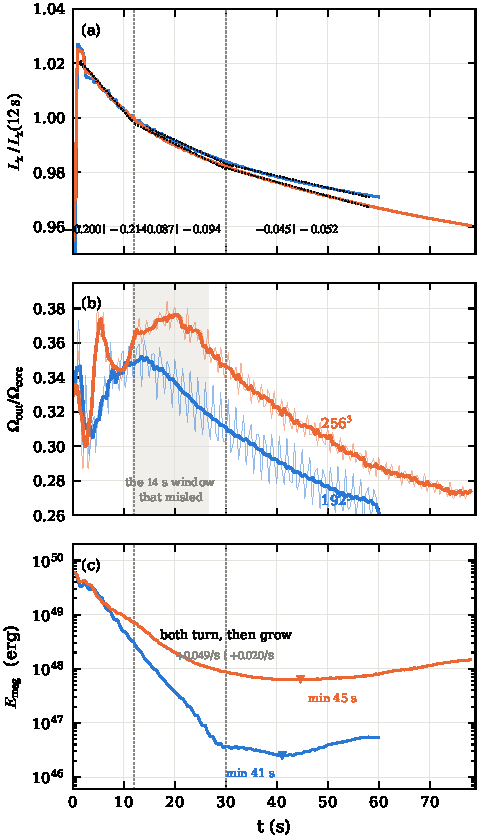
\includegraphics[width=0.62\textwidth]{figures/late_convergence.pdf}
\caption{The three results. \textbf{(a)} $L_z$ normalised at $t = 12$\,s, with
the three braking regimes fitted; the numbers along the bottom are
$192^3\,|\,256^3$ in percent per second, and the dashed verticals are the
regime boundaries. \textbf{(b)} The differential rotation. The finer grid
begins to steepen about $6$\,s late, then steepens faster; the shaded band is
the $14$\,s window over which that lag reads as a disagreement.
\textbf{(c)} Magnetic energy, the one panel that does not converge. The $192^3$
field diagnostics stop at $t = 12$\,s; the isolated point at $t = 38.5$\,s is
the single late instant that was processed, and is drawn as a marker because
that is all it is.}
\label{fig:late}
\end{figure}

%======================================================================
\section{The field, before and after}

Before the numbers, the pictures. Fig.~\ref{fig:seq192} is what the ordered
field does at $192^3$: axisymmetric circles of $\Btor$ in the equatorial cut at
$t=0$, an $m=1$ deformation growing through $t \simeq 2$--$4$\,s, filamentation
at saturation, and a disordered remnant afterwards. The poloidal row below it
starts almost empty --- the initial poloidal field is three decades below the
toroidal one --- and fills in as the instability converts one into the other.

\begin{figure}[t]
\centering
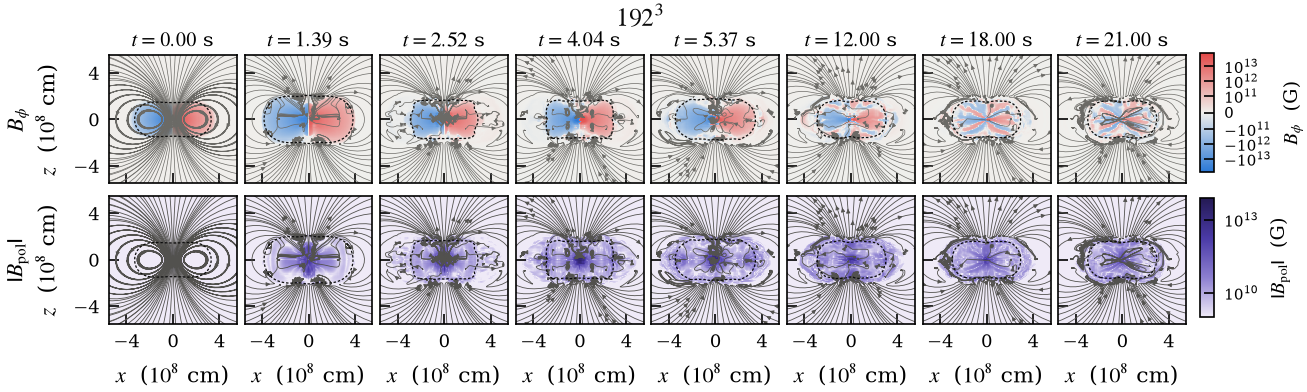
\includegraphics[width=\textwidth]{figures/field_sequence_192.png}
\caption{$192^3$, $t = 0$ to $21$\,s. \textbf{Top:} equatorial cut $z=0$, where
$\Btor$ lies in the plane, so the streamlines \emph{are} the toroidal field
lines --- circles while the star is axisymmetric, and their departure from
circles is the instability. \textbf{Bottom:} meridional cut $y=0$, where the
in-plane field \emph{is} the poloidal one. Colour is $\Btor$ and $|\Bpol|$,
both starting at $10^{10}$\,G so the two rows share a threshold in gauss. The
dashed contour is $\rho = 10^{6}$\,g\,cm$^{-3}$.}
\label{fig:seq192}
\end{figure}

\begin{figure}[t]
\centering
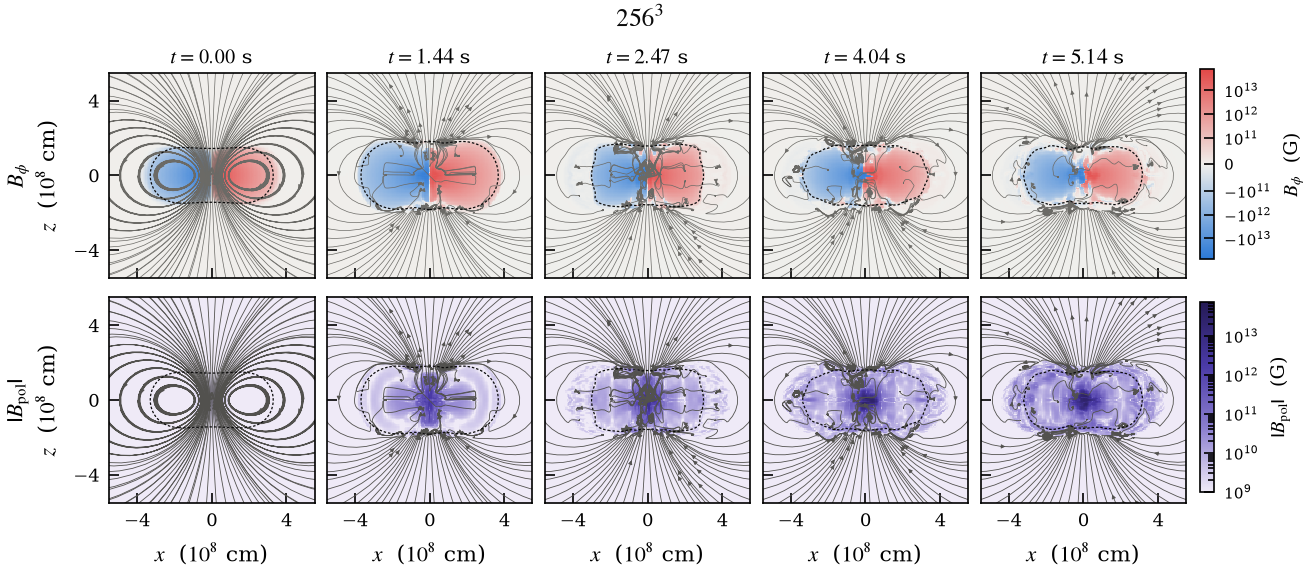
\includegraphics[width=\textwidth]{figures/field_sequence_256.png}
\caption{$256^3$, same planes, same colour scales, same threshold as
Fig.~\ref{fig:seq192} --- the two are meant to be compared panel by panel.
\textbf{This sequence stops at $t = 5.14$\,s}, the end of the growth phase,
because those are the only instants for which slices have been extracted. It
therefore covers none of the window this report is about. Extending it is the
obvious companion to Sec.~\ref{sec:residual}: a slice at $t \simeq 58$\,s would
show directly whether the residual field that fails to converge is organised or
turbulent, which is the physical question underneath the two readings offered
there.}
\label{fig:seq256}
\end{figure}

The comparison that matters for this report is not visible in either figure.
Both stop before or barely into the window where the two grids disagree about
the residual, and the disagreement is a factor of $25$ in energy --- large
enough that it should be plainly visible in a slice, as either a different
field strength or a different degree of organisation. That figure is the one
piece of evidence this report is missing.

%======================================================================
\section{The braking of $L_z$ converges}

This is the strongest result of the comparison, and it is the one that matters
most for the physics, because it is what identifies the transport.

\begin{table}[h]
\centering\small
\begin{tabular}{lrrl}
\toprule
$\mathrm{d}\ln L_z/\mathrm{d}t$ & $192^3$ & $256^3$ & agreement \\
\midrule
$t = 1.5$--$11.9$\,s \quad toroidal field alive & $-0.1996\%$/s & $-0.2144\%$/s & $7\%$ \\
$t = 12$--$30$\,s \quad\;\, field decaying & $-0.0873\%$/s & $-0.0935\%$/s & $7\%$ \\
$t = 30$--$58$\,s \quad\;\, residual & $-0.0446\%$/s & $-0.0523\%$/s & $15\%$ \\
\bottomrule
\end{tabular}
\caption{Three regimes, each braking at about half the rate of the one before,
and the two grids agree on all three.}
\label{tab:braking}
\end{table}

There is no explicit viscosity and no explicit resistivity in these runs, so
nothing else in the scheme brakes anything. The star loses angular momentum
twice as fast while the ordered toroidal field exists as it does afterwards,
and half as fast again once even the decaying field has gone. That factor of
two, repeated, is the signature of magnetic transport, and it is now measured
at two resolutions instead of one.

The third regime is new here --- Report~I described two. With the baseline
extended it is clear that the braking does not simply switch from ``fast'' to
``slow'' when the field dies but continues to weaken as the field weakens,
which is what a magnetic mechanism should do and what a numerical one need not.

\paragraph{What this does not establish.} The rates agree between the grids;
that does not make them physical. Both runs brake through whatever transport
the scheme supplies, and if a component of that is numerical it may well
converge at the same rate as the physical part. The argument for the magnetic
identification is the \emph{correlation with the field}, not the convergence;
convergence only removes the worry that the correlation was a coarse-grid
accident.

%======================================================================
\section{The steepening converges --- over a long enough baseline}
\label{sec:steep}

The differential rotation is the property the configuration depends on: a
$2\,\Msun$ white dwarf exists here only because $\Omega$ falls steeply outwards.
Report~I found that the profile not only survives but steepens, and flagged the
amplitude as unconverged.

\begin{table}[h]
\centering\small
\begin{tabular}{lrrl}
\toprule
$12$--$15$\,s $\to$ $55$--$58.3$\,s & $192^3$ & $256^3$ & \\
\midrule
$L_z$ & $-2.6\%$ & $-2.9\%$ & converged \\
$\Oout$ & $-15.3\%$ & $-14.9\%$ & converged ($3\%$) \\
$\Oout/\Ocore$ & $\mathbf{-22.6\%}$ & $\mathbf{-20.3\%}$ & \textbf{converged ($10\%$)} \\
$\Ocore$ & $+9.4\%$ & $+6.7\%$ & same sign \\
$L_z^{\mathrm{outer}}/L_z^{\mathrm{inner}}$ & $-10.6\%$ & $-6.2\%$ & same sign \\
\bottomrule
\end{tabular}
\caption{The steepening over $46$\,s. The amplitude converges to $10\%$ and the
outer-shell spin-down to $3\%$.}
\label{tab:steep}
\end{table}

\subsection{A convergence test shorter than the lag measures the lag}

The amplitude looked irreducibly resolution-dependent over shorter windows, and
the reason is worth recording because it is a trap that will recur in this
problem.

\begin{table}[h]
\centering\small
\begin{tabular}{lrr}
\toprule
change in $\Oout/\Ocore$ & $192^3$ & $256^3$ \\
\midrule
$t = 12 \to 18$\,s & $-3.2\%$ & $\mathbf{+2.1\%}$ \\
$t = 18 \to 24$\,s & $-5.1\%$ & $-3.0\%$ \\
$t = 24 \to 30$\,s & $-4.5\%$ & $\mathbf{-5.6\%}$ \\
$t = 30 \to 38$\,s & $-3.8\%$ & $\mathbf{-5.2\%}$ \\
\midrule
total over a $14$\,s baseline & $-8.2\%$ & $-1.0\%$ \\
total over a $46$\,s baseline & $-22.6\%$ & $-20.3\%$ \\
\bottomrule
\end{tabular}
\caption{The finer grid is still flat --- rising, even --- while the coarse
grid has already begun, and then steepens faster. The last two rows are the
same comparison over two baselines: a factor of eight apart at $14$\,s, ten
percent apart at $46$\,s.}
\label{tab:lag}
\end{table}

Neither number is wrong. The short baseline simply does not contain the onset,
and a delayed effect measured over a window shorter than its delay is
indistinguishable from an absent effect --- and, if the lagging curve happens to
drift the other way first, from an effect of the opposite sign.

This cost two wrong conclusions in successive drafts of Report~I: first that
the steepening was a coarse-grid artefact, then that its direction was real but
its amplitude was not. Both were stated with the numbers that supported them,
and both were wrong for the same reason.

The general form is uncomfortable, because the lag is not known in advance and
is not obviously bounded. Here it is $6$\,s against a $1.5$\,s pulsation and a
$2.4$\,s Alfv\'en time --- a few dynamical times, which is reassuring but is a
measurement, not a principle. Any future convergence test in this problem needs
a baseline long enough that a plausible lag is a small fraction of it.

%======================================================================
\section{The field stops decaying and regrows --- on both grids}
\label{sec:residual}

This began as the one section where extending the baseline made the
disagreement worse. It has become the one positive result in the campaign:
something the star \emph{does}, rather than something it loses.

\begin{table}[h]
\centering\small
\begin{tabular}{lrrl}
\toprule
& $192^3$ & $256^3$ & \\
\midrule
minimum of $\Emag$ & $t = 41.1$\,s & $t = 44.7$\,s & \textbf{both turn} \\
$\Emag$ at the minimum (erg) & $2.54\times10^{46}$ & $6.35\times10^{47}$ & $\times 24.5$ apart \\
growth, whole rise & $+0.0485$/s & $+0.0282$/s & \emph{coarse grid faster} \\
\quad settled rate, $t>55$\,s & --- & $+0.035$/s & $e$-fold $29$\,s \\
minimum to end of run & $+114\%$ & $+124\%$ & \\
$\max|B|$ over the rise & $+45\%$ & $+107\%$ & \\
\bottomrule
\end{tabular}
\caption{The minima are located by fitting a parabola to $\ln\Emag$ over
$t = 25$--$55$\,s, so the $1.5$\,s pulsation does not set the answer. That the
turnaround exists is converged; nothing quantitative about it is.}
\label{tab:turn}
\end{table}

\paragraph{What is converged.} Both runs decay, reach a minimum within $4$\,s
of each other, and then grow monotonically to the end of the available data.
The mechanism is not exotic and it is available: the differential rotation
survives and is still \emph{steepening} (Sec.~\ref{sec:steep}), so there
is free shear energy, and winding residual poloidal field into toroidal is the
most ordinary thing a shear flow can do to a magnetic field.

\paragraph{The rise is exponential and steady.} Carried to $t = 78$\,s, the
$256^3$ growth settles: fitting $\ln\Emag$ over $t = 55$--$65$ gives
$+0.0354$\,s$^{-1}$ and over $t = 65$--$78$ gives $+0.0349$\,s$^{-1}$. Two
independent ten-second windows agreeing to $1.5\%$ is an exponential, not a
transient, with an $e$-folding of $29$\,s. Over the whole rise $\Emag$ more
than doubles and the peak field goes from $4.05$ to $8.37\times10^{12}$\,G.

\paragraph{An oscillation would now have to be implausibly slow.} The rise has
been monotone for $33$\,s. A sinusoid accelerating away from its minimum
inflects at a quarter period, so explaining this needs $P > 133$\,s --- $280$
dynamical times, or $89$ of the star's own pulsation periods. Without a named
mode at that period the reading is hard to sustain.

\paragraph{The two grids are converging.} The gap in $\Emag$ narrows
monotonically: $24.5$ at the minimum, $16.1$ at $t = 51$\,s, $14.1$ at
$t = 58$\,s, which is as far as the $192^3$ run goes. A level set by the mesh
would hold its ratio; a level the two runs are both climbing towards would
close, and closing is what is observed. Extrapolating the two rates naively has
them meeting near $t \simeq 190$\,s, far beyond either run.

\paragraph{What is still not converged.} The rate itself. Over the window both
grids cover, the coarse one grows about $2.4$ times faster --- the same
direction, and a similar factor, as the decay rate before it, which fell from
$0.282$ to $0.141$\,s$^{-1}$ under the same refinement. So the phenomenon is
robust and its timescale is not.

\paragraph{A prediction that failed, recorded because it was registered.}
Before this data existed it was written down that the $192^3$ would turn
\emph{later} and \emph{more weakly}, on the reasoning that more numerical
dissipation should delay the point where regeneration overtakes decay. It
turns $3.6$\,s \textbf{earlier} and grows $2.5$ times \textbf{faster}. The
prediction was wrong in both directions. What it was testing --- whether the
turnaround appears at all on the coarse grid --- came out yes, which is why
the section above survives.

The failure is informative about the mechanism. If the regrowth were a dynamo
running against numerical dissipation, less dissipation should mean earlier
and stronger, and the opposite is observed. A reading consistent with the
numbers is that both grids are winding toward a saturation level, and the one
starting $25$ times lower has further to travel and so climbs faster in
relative terms --- but the gap only narrows from $25$ to $16$ over the
available window, so they are not visibly converging on a common level either.

%======================================================================
\section{What changes in Report~I}

\begin{enumerate}\itemsep3pt
\item \textbf{Strengthened.} The magnetic identification of the transport. Two
      grids, three regimes, agreement of $7$--$15\%$.
\item \textbf{Strengthened.} The steepening of the differential rotation, now
      converged in amplitude as well as direction.
\item \textbf{Weakened.} Everything about the end state of the field. The
      residual is a mesh floor and the destruction factor is an upper bound.
      Report~I's Table~4 should be read with that in mind: its mass, radii and
      rotation rows are measurements, its field rows are bounds.
\item \textbf{New caveat.} Convergence tests in this problem need baselines
      longer than the inter-grid lag, and the lag is only known afterwards.
\end{enumerate}

%======================================================================
\section*{Status and next steps}

$192^3$: complete, $t = 60$\,s, field diagnostics processed to $t = 12$\,s plus
the single instant at $38.5$\,s. \quad $256^3$: $t = 58.2$\,s, all $164$
plotfiles processed. A final window to $60$\,s is queued; nothing here depends
on it.

The cheapest thing that would sharpen this report is not more physical time but
the missing $192^3$ field data: processing its plotfiles between $t = 12$ and
$60$\,s would turn the single point in Fig.~\ref{fig:late}c into a curve and
make the residual comparison a proper one rather than a snapshot against a
mean. It costs no new simulation.

Beyond that, the run that would test the interpretation directly is a
genuinely mixed field --- comparable poloidal and toroidal energy, rather than
the $10^{-7}$ ratio used here. A toroidal-dominated field is the textbook
unstable case and behaved like one; the twisted-torus configuration is the one
expected to survive, and it is the geometry the equilibrium literature on
super-Chandrasekhar white dwarfs does not construct.

\vspace{0.6em}
\noindent
Inputs, submission scripts, diagnostic tools, data and figure code are under
version control in the \texttt{WD\_MAG} repository. The data behind every number
here is \texttt{investigations/bt\_bp\_256\_long.csv} ($164$ rows, $t = 0$ to
$58.2$\,s) and \texttt{investigations/rotation\_192.csv}.

\end{document}
